\documentclass[14pt,a4paper]{extarticle}
\usepackage[T2A]{fontenc}
\usepackage[utf8]{inputenc}
\usepackage[english,russian]{babel}
\usepackage{lmodern}
\usepackage{geometry}
\usepackage{array}
\usepackage{tabularx}
\usepackage{longtable}
\usepackage{ltablex}
\usepackage{booktabs}
\usepackage{hyperref}
\usepackage{indentfirst}
\usepackage{microtype}
\usepackage{graphicx}
\usepackage{setspace}
\usepackage{listings}
\usepackage{graphicx}
\usepackage{caption}
\usepackage{float}
\usepackage{tocloft}
\usepackage{titlesec}
\usepackage{newtxtext,newtxmath}

\titleformat{\section}        % форматируем \section
  {\normalfont\bfseries}      % стиль: обычный + жирный
  {\thesection.}              % номер секции с точкой
  {2mm}                       % расстояние между номером и текстом
  {}                           % перед заголовком можно добавить что-то
\titlespacing*{\section}{1.5cm}{*3}{*1}  % {отступ слева}{отступ сверху}{отступ снизу}

\captionsetup{justification=centering}
\renewcommand{\ttdefault}{cmtt}
\keepXColumns
\setlength{\parindent}{3em}
\newgeometry{left=2.5cm,right=2.5cm,top=3cm,bottom=2.5cm}

\renewcommand{\contentsname}{\hspace*{4em}{\smallСодержание}}
\setlength{\cftbeforesecskip}{0.5em}
\renewcommand{\cftsecleader}{\cftdotfill{\cftdotsep}}
\renewcommand{\cftsecaftersnum}{.\hspace{2mm}}

\title{Отчёт по дисциплине "Системная инженерия"}
\author{Выполнил студент группы М-РИТ-25-1, Станиславчук Сергей}

\begin{document}

\setstretch{1.5}
\noindent
\begin{minipage}[t]{0.01\textwidth}
    \includegraphics{~/programmer/++Programmer/5_1/LSTU.jpg}
\end{minipage}%
\begin{minipage}[c]{1.1\linewidth}
    \centering
    {\small
    МИНИСТЕРСТВО НАУКИ И ВЫСШЕГО ОБРАЗОВАНИЯ РФ \\[1em]
    ФЕДЕРАЛЬНОЕ ГОСУДАРСТВЕННОЕ БЮДЖЕТНОЕ \\
    ОБРАЗОВАТЕЛЬНОЕ УЧРЕЖДЕНИЕ ВЫСШЕГО ОБРАЗОВАНИЯ \\
    «ЛИПЕЦКИЙ ГОСУДАРСТВЕННЫЙ ТЕХНИЧЕСКИЙ УНИВЕРСИТЕТ»
    }
\end{minipage}%

\vspace{3em}

\noindent
\hspace{1em}%
\begin{minipage}[t]{0.8\textwidth}
\textbf{Институт} \hspace{2em} компьютерных наук \\
\textbf{Кафедра} \hspace{2em} автоматизированных систем управления
\end{minipage}


\vspace{6em}

\begin{center}
\textbf{Домашнее задание №4} \\
по дисциплине \\ <<Системная инженерия>>
\end{center}

\vspace{6em}

\noindent
\begin{tabular*}{\textwidth}{@{\extracolsep{\fill}} l c r }
    Студент М-РИТ-25-1 & \makebox[4cm]{\hrulefill} & Станиславчук С.М. \\[2em]
Руководитель & \\
Профессор, канд. тех. наук & \makebox[4cm]{\hrulefill} & Качановский Ю.П. \\
\end{tabular*}

\vfill
\begin{center}
    Липецк, 2026
\end{center}

\thispagestyle{empty}

\newpage
\tableofcontents
\newpage

\section{Задание кафедры}
\begin{sloppypar}
    1. Повторить вербальное (словесное) описание проектируемой системы
    2. Для моделирования структуры системы построить диаграмму определения блоков верхнего уровня (Top Level) и 1-2 диаграммы определения блоков для основной части (основных частей) системы, используя связи объединений (физических и логических) и обобщения (по возможности).
    3. На отдельной диаграмме (диаграммах) описания блоков определить структурные и поведенческие характеристики основных блоков.
    4. Построить модель взаимодействия основных частей системы (1-2 диаграммы внутренней структуры блоков) с указанием портов и потоков элементов между ними, а также интерфейсов (по возможности).
\end{sloppypar}

\section{Описание проектируемой системы}

Система корпоративного обмена сообщениями в реальном времени
Предназначена для организации защищённой текстовой и голосовой связи внутри корпоративной сети без использования внешних централизованных сервисов, с минимальной зависимостью от внешней инфраструктуры.

Объектом управления является коммуникационная инфраструктура организации, включающая серверы, клиентские устройства пользователей и сетевые каналы передачи данных. С помощью клиентского приложения пользователь получает доступ к текстовым чатам, голосовым каналам и передаче файлов. Управление системой осуществляется через интерфейс, позволяющий создавать каналы связи, отправлять сообщения, подключаться к голосовым сессиям и обмениваться данными.

Внутри системы осуществляется постоянное установление и поддержание соединений между клиентами и сервером. Сервер обрабатывает входящие сообщения, управляет сессиями пользователей и обеспечивает маршрутизацию данных. Передача текстовых сообщений происходит в режиме реального времени, а голосовая связь реализуется через потоковую передачу данных с учётом минимизации задержек.

Система также выполняет контроль доступа и защиту данных. Аутентификация пользователей, шифрование передаваемой информации и разграничение прав доступа обеспечивают безопасность взаимодействия. При передаче файлов система контролирует целостность данных и управляет их доставкой между участниками.

Таким образом, система обеспечивает автоматизированное управление процессом корпоративной коммуникации, поддерживая стабильный обмен данными, безопасность и высокую скорость взаимодействия внутри сети организации.

\section{Диаграммы блоков}

Диаграмма блоков верхнего уровня представлена на рисунке 1.

\begin{figure}[H]
    \label{fig:1}
    \centering
    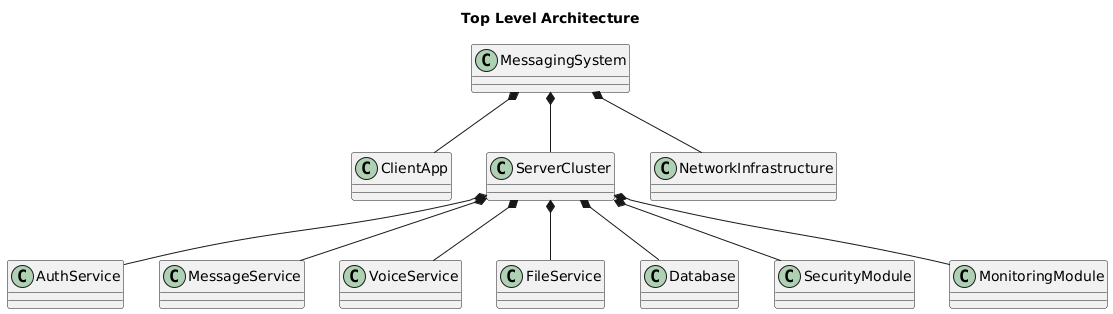
\includegraphics[width=0.78\textwidth]{BDD.png}
    \refstepcounter{figure}
    \caption*{Рисунок \thefigure\ — Диаграмма блоков верхнего уровня}
\end{figure}

Диаграмма блоков серверной части представлена на рисунке 2.

\begin{figure}[H]
    \label{fig:2}
    \centering
    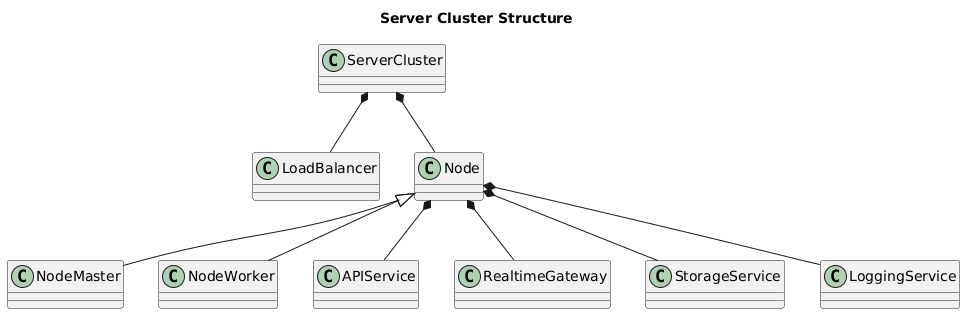
\includegraphics[width=0.78\textwidth]{bdd_server.png}
    \refstepcounter{figure}
    \caption*{Рисунок \thefigure\ — Диаграмма блоков серверной части}
\end{figure}

Диаграмма блоков клиентской части представлена на рисунке 3.

\begin{figure}[H]
    \label{fig:3}
    \centering
    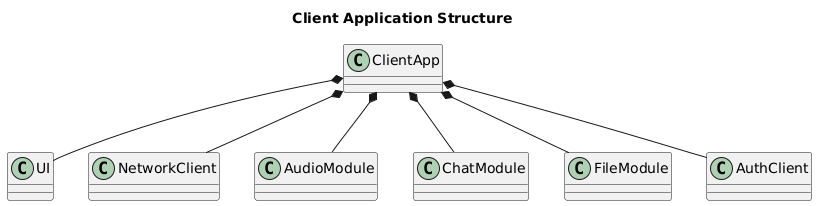
\includegraphics[width=0.78\textwidth]{bdd_client.png}
    \refstepcounter{figure}
    \caption*{Рисунок \thefigure\ — Диаграмма блоков клиентской части}
\end{figure}

\section{Структурные и поведенческие характеристики блоков}

Диаграмма блоков серверной части представлена на рисунке 4.

\begin{figure}[H]
    \label{fig:4}
    \centering
    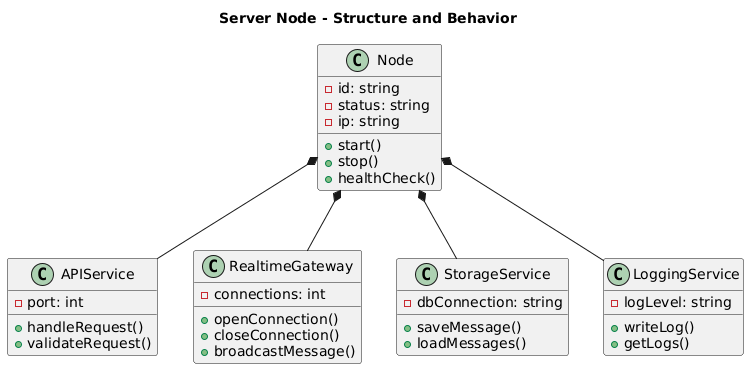
\includegraphics[width=0.78\textwidth]{3_server.png}
    \refstepcounter{figure}
    \caption*{Рисунок \thefigure\ — Диаграмма блоков серверной части}
\end{figure}

Диаграмма блоков клиентской части представлена на рисунке 5.

\begin{figure}[H]
    \label{fig:5}
    \centering
    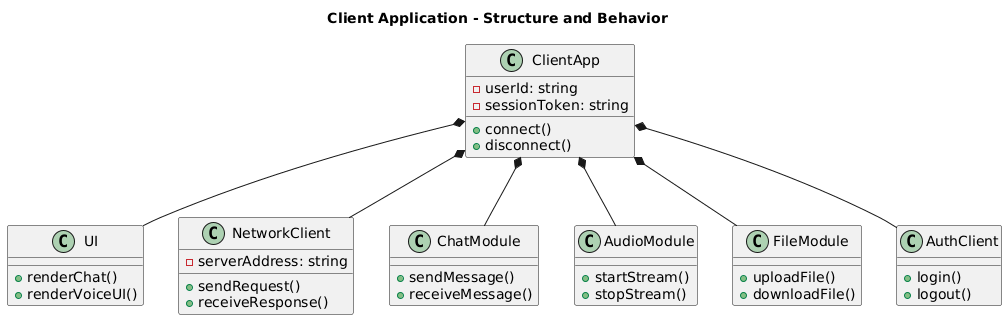
\includegraphics[width=0.78\textwidth]{3_client.png}
    \refstepcounter{figure}
    \caption*{Рисунок \thefigure\ — Диаграмма блоков клиентской части}
\end{figure}

\section{Модель взаимодействия основных частей системы}

Модель взаимодействия основных частей системы представлена на рисунке 6.

\begin{figure}[H]
    \label{fig:6}
    \centering
    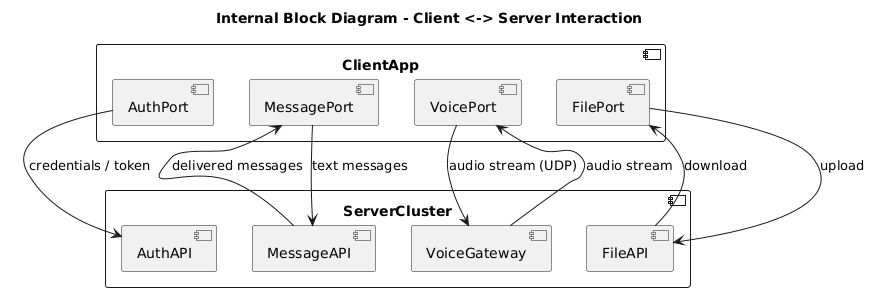
\includegraphics[width=0.78\textwidth]{4_client-server.png}
    \refstepcounter{figure}
    \caption*{Рисунок \thefigure\ — Модель взаимодействия основных частей системы}
\end{figure}

\end{document}
